\section{零阶随机梯度方法}
\label{sec:zo-method}

前两节构造了各种方向估计。接下来要弄清：把它们放进迭代后，算法实际在优化什么，步长和扰动尺度怎样定，遇到约束怎么办，最后交出什么结果？

\subsection{基本迭代}
\label{sec:zo-basic}

\paragraph{主要思想}
第~\ref{chap:stochastic-gradient-methods}章的随机更新沿随机方向$\hat{\bm{g}}^{(t)}$的负向走一步。它能用的原因是，这个方向平均起来指向某个函数的梯度。零阶方法沿用这个更新，只是$\hat{\bm{g}}^{(t)}$由函数值算出：
\begin{equation}
 \bm{x}^{(t+1)}=\bm{x}^{(t)}-\alpha^{(t)}\hat{\bm{g}}^{(t)},\qquad
 \hat{\bm{g}}^{(t)}=\frac{n}{2\delta}\bigl(y_+^{(t)}-y_-^{(t)}\bigr)\bm{u}^{(t)}.
 \label{eq:zo-update}
\end{equation}
这是\term{零阶随机梯度方法}（zeroth-order stochastic gradient method）的双点形式，其他估计器可以替换第二式。一轮的流程如图~\ref{fig:zo-flow}所示。

\begin{BookInlineFigure}
  \centering
  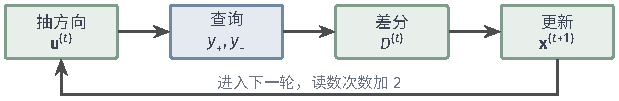
\includegraphics[width=105mm]{figures/05-optimization/05-stochastic-optimization/tikz/zo-flow/figure.pdf}
  \caption{双点零阶方法的一轮。绿框是算法内部的计算，蓝框是向黑箱提交的查询。每轮两次函数读数，查询预算按读数次数累计。}
  \label{fig:zo-flow}
\end{BookInlineFigure}

更新形式都一样，算法朝哪里走却由估计器的条件均值决定，不能只看形式。式~\eqref{eq:zo-update}的条件均值是$\nabla f^{\mathrm{B}}_{\delta}(\bm{x}^{(t)})$，所以它是平滑目标上的随机梯度方法，不是原目标上的。

\needspace{6\baselineskip}
\paragraph{变量}
\begin{itemize}
 \item $\bm{x}^{(t)}\in\mathbb{R}^n$：当前迭代点。
 \item $\bm{u}^{(t)}\in\bm{S}$：本轮的单位方向，$n$维。
 \item $y_\pm^{(t)}$：两次读数，标量。
 \item $D^{(t)}=(y_+^{(t)}-y_-^{(t)})/(2\delta)$：差商，标量。
 \item $\hat{\bm{g}}^{(t)}\in\mathbb{R}^n$：方向估计。
 \item $\alpha$、$\delta$：步长与扰动半径，取常数。
 \item $Q$：已用读数次数。
\end{itemize}

\paragraph{初始化}
取起点$\bm{x}^{(0)}$，选定$\alpha$、$\delta$和读数预算$Q_{\max}$，令$Q=0$。例中目标是贯穿例~\eqref{eq:zo-example}，读数带独立噪声，并取
\[
 \bm{x}^{(0)}=(9,1),\quad\alpha=0.05,\quad\delta=0.5,\quad Q_{\max}=6.
\]

\needspace{6\baselineskip}
\paragraph{每轮更新}
下面的数值用事先给定的方向和噪声，便于逐项核对。
\begin{enumerate}
 \item 抽取方向$\bm{u}^{(t)}$。例中第一轮$\bm{u}^{(0)}=(0.6,0.8)$，第二轮$\bm{u}^{(1)}=(0.8,-0.6)$，第三轮$\bm{u}^{(2)}=(0.28,0.96)$。
 \item 查询$\bm{x}^{(t)}\pm\delta\bm{u}^{(t)}$，$Q$增加$2$。例中第一轮两个查询点是$(9.3,1.4)$和$(8.7,0.6)$，真实函数值为$52.065$和$39.465$，噪声分别为$+0.1$和$-0.1$，读数是
 \[
  y_+^{(0)}=52.165,\qquad y_-^{(0)}=39.365.
 \]
 \item 由式~\eqref{eq:zo-update}算差商和方向估计。例中$2\delta=1$，$n=2$，第一轮结果是
 \[
  D^{(0)}=12.8,\qquad\hat{\bm{g}}^{(0)}=2\cdot12.8\cdot(0.6,0.8)=(15.36,\ 20.48).
 \]
 \item 由式~\eqref{eq:zo-update}沿$-\hat{\bm{g}}^{(t)}$走步长$\alpha$。例中第一轮得到
 \[
  \bm{x}^{(1)}=(9,1)-0.05\,(15.36,20.48)=(8.232,\ -0.024).
 \]
\end{enumerate}

第二轮从$\bm{x}^{(1)}$出发，查询点是$(8.632,-0.324)$和$(7.832,0.276)$，噪声是$-0.1$和$+0.1$，读数和结果为
\[
 y_+^{(1)}\approx37.628,\quad y_-^{(1)}\approx31.113,\quad D^{(1)}\approx6.515,
\]
\[
 \hat{\bm{g}}^{(1)}\approx(10.424,\ -7.818),\qquad\bm{x}^{(2)}\approx(7.711,\ 0.367).
\]

第三轮查询点是$(7.851,0.847)$和$(7.571,-0.113)$，噪声是$+0.05$和$+0.15$，读数和结果为
\[
 y_+^{(2)}\approx34.095,\quad y_-^{(2)}\approx28.866,\quad D^{(2)}\approx5.229,
\]
\[
 \hat{\bm{g}}^{(2)}\approx(2.928,\ 10.040),\qquad\bm{x}^{(3)}\approx(7.564,\ -0.135).
\]

迭代在$Q$达到$Q_{\max}$时结束。例中三轮用完$6$次读数，最终得到$\bm{x}^{(3)}\approx(7.564,-0.135)$，真实目标值约$28.69$，从$45$下降了三分之一多。第二轮的梯度第二分量只有$-0.216$，估计的第二分量却是$-7.818$，$x_2$从$-0.024$跳到$0.367$，这种摆动是单方向估计的常态。继续运行的结果见图~\ref{fig:zo-paths}。

\begin{BookInlineFigure}
  \centering
  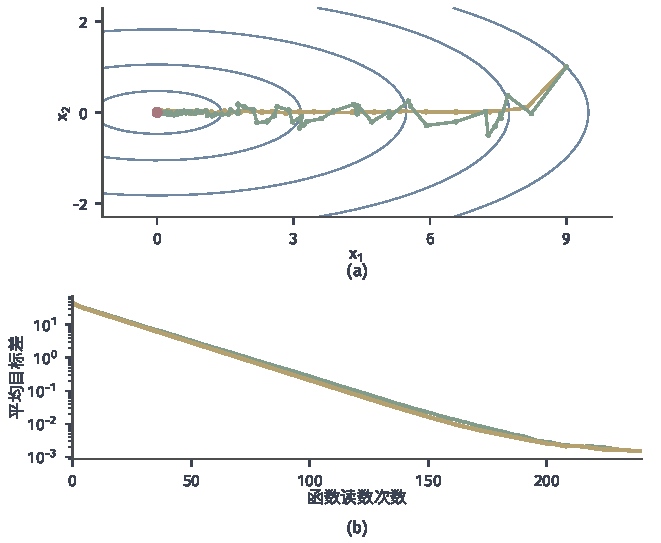
\includegraphics[width=112mm]{figures/05-optimization/05-stochastic-optimization/matplotlib/zo-paths/figure.pdf}
  \caption{贯穿例上的零阶迭代，读数噪声标准差$0.1$。(a)绿线是双点球面方法的一次运行，$\alpha=0.05$，$\delta=0.5$，前三轮即正文手算的数据，共$120$轮；黄线是中心坐标差分的梯度下降，$\alpha=0.1$，$h=0.5$，共$60$轮；蓝线是等高线，红点是解。(b)$200$次运行的平均目标差，横轴是函数读数次数。}
  \label{fig:zo-paths}
\end{BookInlineFigure}

图~\ref{fig:zo-paths}(a)中绿线抖动，黄线平稳，但按读数次数算两者几乎重合，如图~\ref{fig:zo-paths}(b)。这里两者的步长不同：单方向估计的步长要比完整梯度小一个与$n$相关的倍数，原因在第~\ref{sec:zo-step-scale}节说明。

\paragraph{多方向平均}
每轮抽$m$个独立方向，分别计算估计后取平均，是最常见的变体，一轮用$2m$次读数：
\begin{equation}
 \hat{\bm{g}}^{(t)}=\frac{1}{m}\sum_{j=1}^{m}\frac{n}{2\delta}\bigl(y_{j,+}^{(t)}-y_{j,-}^{(t)}\bigr)\bm{u}_j^{(t)}.
 \label{eq:zo-multi-direction}
\end{equation}
条件均值不变，方差变成$1/m$。例中第一轮若用$\bm{u}_1=(0.6,0.8)$和$\bm{u}_2=(0.8,-0.6)$两个方向，不计噪声时，两个估计是
\[
 (15.12,\ 20.16),\qquad(2.88,\ -2.16).
\]
它们的平均恰为$(9,9)$，这时$\bm{x}^{(1)}=(8.55,0.55)$。两个方向正交且数量等于维数，对二次函数恰好拼出了完整梯度。

\paragraph{一步分析：有偏与无偏两条路}
把估计器代入迭代，有两种分析方式，对应前面的两种读法。先假设$\nabla f$是$L$-Lipschitz的，第一种直接看原目标。

\begin{lemma}[单步下降]
\label{lem:zo-one-step}
设$\bm{x}^+=\bm{x}-\alpha\hat{\bm{g}}$，$\nabla f$是$L$-Lipschitz的。若$\hat{\bm{g}}$的条件均值是$\nabla f(\bm{x})+\bm{b}$，且$\lVert\bm{b}\rVert_2\leq\beta$，则
\begin{equation}
 \mathbb{E}[f(\bm{x}^+)\mid\bm{x}]\leq f(\bm{x})-\frac{\alpha}{2}\lVert\nabla f(\bm{x})\rVert_2^2+\frac{\alpha}{2}\beta^2+\frac{L\alpha^2}{2}\mathbb{E}\bigl[\lVert\hat{\bm{g}}\rVert_2^2\mid\bm{x}\bigr].
 \label{eq:zo-biased-step}
\end{equation}
若$\hat{\bm{g}}$的条件均值是$\nabla f^{\mathrm{B}}_{\delta}(\bm{x})$，则
\begin{equation}
 \mathbb{E}[f^{\mathrm{B}}_{\delta}(\bm{x}^+)\mid\bm{x}]\leq f^{\mathrm{B}}_{\delta}(\bm{x})-\alpha\lVert\nabla f^{\mathrm{B}}_{\delta}(\bm{x})\rVert_2^2+\frac{L\alpha^2}{2}\mathbb{E}\bigl[\lVert\hat{\bm{g}}\rVert_2^2\mid\bm{x}\bigr].
 \label{eq:zo-unbiased-step}
\end{equation}
\end{lemma}

\begin{proof}
由下降引理，对$L$-光滑函数$\psi$，
\[
 \psi(\bm{x}^+)\leq\psi(\bm{x})-\alpha\langle\nabla\psi(\bm{x}),\hat{\bm{g}}\rangle+\frac{L\alpha^2}{2}\lVert\hat{\bm{g}}\rVert_2^2.
\]
取$\psi=f$并取条件期望，内积项变为$-\alpha\lVert\nabla f\rVert_2^2-\alpha\langle\nabla f,\bm{b}\rangle$。再用
\[
 -\langle\nabla f,\bm{b}\rangle\leq\frac12\lVert\nabla f\rVert_2^2+\frac12\beta^2,
\]
得式~\eqref{eq:zo-biased-step}。

取$\psi=f^{\mathrm{B}}_{\delta}$，由引理~\ref{lem:zo-smoothing-properties}，它也是$L$-光滑的，内积项的条件期望是$-\alpha\lVert\nabla f^{\mathrm{B}}_{\delta}\rVert_2^2$，得式~\eqref{eq:zo-unbiased-step}。
\end{proof}

两式对比可以看出两种分析的差别。式~\eqref{eq:zo-biased-step}留下了偏差项$\tfrac{\alpha}{2}\beta^2$，它每步都存在，累加后构成不会随步数消失的误差。式~\eqref{eq:zo-unbiased-step}没有偏差项，账记在平滑目标上，代价是结论说的是$f^{\mathrm{B}}_{\delta}$，要回到$f$还须另算，这留给第~\ref{sec:zo-original-error}节。

\subsection{步长与扰动尺度}
\label{sec:zo-step-scale}

这里有两个旋钮。步长$\alpha$决定参数实际走多远，扰动尺度$\delta$决定在多大的邻域里比较函数值。两者的量纲都不同：改变$\delta$不移动$\bm{x}$，只改变估计的性质。

\paragraph{步长的上限}
由式~\eqref{eq:zo-noisy-moment}，二阶矩中有$2n\lVert\nabla f\rVert_2^2$，比完整梯度的$\lVert\nabla f\rVert_2^2$大$2n$倍。代入式~\eqref{eq:zo-unbiased-step}，要让下降项压住二阶矩项，需要$\alpha\lesssim1/(nL)$。直观地说，估计的长度波动约为梯度的$\sqrt{n}$倍，步长必须相应地收小。

这个步长要与每轮的读数次数放在一起看。完整坐标差分的步长是$1/L$，但每轮要$2n$次读数；单方向的步长是$1/(nL)$，每轮$2$次读数。按读数次数算，两者每次读数的“进展”同阶，这就是图~\ref{fig:zo-paths}(b)中两条曲线重合的原因。

贯穿例的手算用了$\alpha=0.05<1/(nL)=1/18$。下一小节定理要求的$\alpha\leq1/(4nL)=1/72$更保守，这是为了在任意光滑函数上保证下降，实际使用时常可放宽。

\paragraph{固定尺度对应固定的平滑目标}
$\delta$固定时，迭代是同一个$f^{\mathrm{B}}_{\delta}$上的随机梯度方法，所以固定步长最终会停在一个噪声水平上。图~\ref{fig:zo-delta-floor}(a)在贯穿例上取$\alpha=0.02$，噪声$\sigma=1$，分别用$\delta=0.1,0.5,2$。

三条曲线下降段相同，稳定后的水平差别很大，$\delta$从$0.1$增大到$0.5$，水平约下降$25$倍。这正是式~\eqref{eq:zo-noisy-moment}中$V$的噪声项$n^2\sigma^2/(2\delta^2)$的$1/\delta^2$规律。这个例子是二次函数，平滑没有引入任何偏差，所以$\delta$越大越好；一般函数上$\delta$还有偏差的代价，第~\ref{sec:zo-tradeoff}节讨论。

\begin{BookInlineFigure}
  \centering
  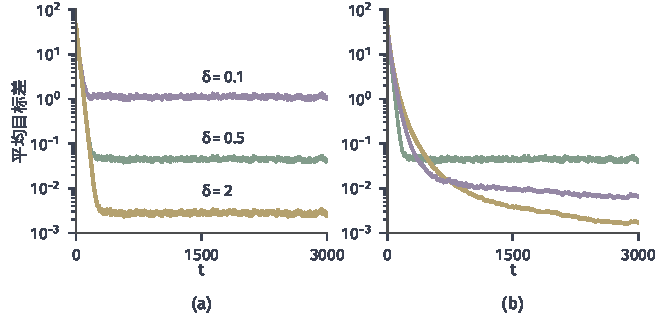
\includegraphics[width=112mm]{figures/05-optimization/05-stochastic-optimization/matplotlib/zo-delta-floor/figure.pdf}
  \caption{贯穿例上双点方法的平均目标差，读数噪声$\sigma=1$，$300$次运行。(a)固定$\alpha=0.02$，紫、绿、黄三线分别为$\delta=0.1,0.5,2$，稳定水平按$1/\delta^2$变化。(b)$\delta=0.5$时固定$\alpha=0.02$（绿）；步长递减$\alpha^{(t)}=0.02/(1+t/100)$（黄）；步长递减较慢、尺度也递减，$\alpha^{(t)}=0.02/(1+t/100)^{0.75}$，$\delta^{(t)}=0.5/(1+t/100)^{0.1}$（紫）。}
  \label{fig:zo-delta-floor}
\end{BookInlineFigure}

\paragraph{递减步长}
要越过这个水平，步长必须递减，这与第~\ref{chap:stochastic-gradient-methods}章的情形相同。图~\ref{fig:zo-delta-floor}(b)的黄线就是在$\delta$固定时让步长递减，曲线继续下降。

\paragraph{逐步缩小尺度要多记两笔}
既然小的$\delta$偏差小，能否让$\delta^{(t)}$随迭代缩小？可以，但目标函数本身在变，分析要多记两笔。

第一笔是目标的变化。第$t$步看的是$f^{\mathrm{B}}_{\delta^{(t)}}$，下一步换成$f^{\mathrm{B}}_{\delta^{(t+1)}}$，累加时不再是同一个函数相减，多出差值$f^{\mathrm{B}}_{\delta^{(t+1)}}-f^{\mathrm{B}}_{\delta^{(t)}}$。若$\delta^{(t+1)}\leq\delta^{(t)}$，由式~\eqref{eq:zo-ball-error}，这个差值的绝对值不超过$L(\delta^{(t)})^2$，一般情形要把它们加起来，$\sum_t(\delta^{(t)})^2$必须受控。

凸函数的情形方便一些。设$\delta_1\leq\delta_2$，$\lambda=\delta_1/\delta_2$。由凸性，
\[
 f(\bm{x}+\delta_1\bm{v})\leq\lambda f(\bm{x}+\delta_2\bm{v})+(1-\lambda)f(\bm{x}).
\]
取期望并用$f\leq f^{\mathrm{B}}_{\delta_2}$，得
\[
 f^{\mathrm{B}}_{\delta_1}\leq f^{\mathrm{B}}_{\delta_2}.
\]
所以缩小半径时平滑目标只降不升，这一笔差值对凸函数不造成损失。

第二笔是方差的变化。$V$里的噪声项是$n^2\sigma^2/(2(\delta^{(t)})^2)$，缩小$\delta$会放大方差，步长必须缩得更快，抵消这部分增长。累加式~\eqref{eq:zo-unbiased-step}可见需要控制的是$\sum_t(\alpha^{(t)})^2V^{(t)}$，因此独立噪声下的标准要求是
\begin{equation}
 \sum_t\alpha^{(t)}=\infty,\qquad
 \sum_t\Bigl(\frac{\alpha^{(t)}}{\delta^{(t)}}\Bigr)^2<\infty,\qquad
 \delta^{(t)}\to0.
 \label{eq:zo-schedule}
\end{equation}
前一个条件保证能走得足够远，后一个条件是随机逼近步长条件的变形\scite{math-robbins1951stochastic}，分母上多了$\delta^{(t)}$，反映差商的噪声放大。图~\ref{fig:zo-delta-floor}(b)的紫线步长递减更慢，尺度也在缩小，两者都使噪声项更大，所以高于黄线。这个二次函数上$\delta$没有偏差可减，缩小尺度没有收益，这也说明$\delta$是否该缩小要看偏差。

\subsection{约束下的查询}
\label{sec:zo-constrained-query}

约束问题要多考虑一件事：不光更新点要可行，查询点也可能需要可行。仿真器在非法参数下可能崩溃，物理实验在限制之外可能损坏设备。

\paragraph{更新可行不等于查询可行}
投影更新
\[
 \bm{x}^{(t+1)}=\Pi_{\bm{C}}\bigl(\bm{x}^{(t)}-\alpha\hat{\bm{g}}^{(t)}\bigr)
\]
保证了迭代点在$\bm{C}$内，但没有限制查询点。以$\bm{C}=[1,9]\times[-1,1]$为例，$\bm{x}=(1,0.4)$在边界上，取$\delta=0.2$，$\bm{u}=(0.6,0.8)$，两个查询点是
\[
 \bm{x}+\delta\bm{u}=(1.12,\ 0.56),\qquad\bm{x}-\delta\bm{u}=(0.88,\ 0.24).
\]
第二个点的$x_1<1$，越出了可行域，如图~\ref{fig:zo-constrained}(a)。投影把迭代点拉回来，却管不到这一步。

\begin{BookInlineFigure}
  \centering
  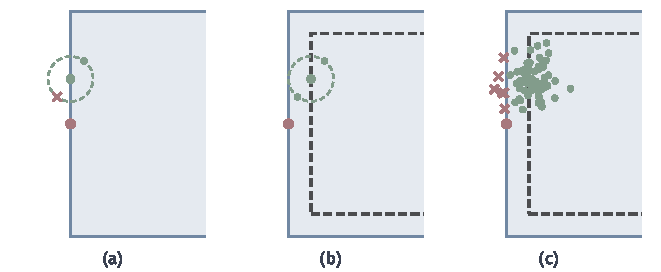
\includegraphics[width=112mm]{figures/05-optimization/05-stochastic-optimization/matplotlib/zo-constrained/figure.pdf}
  \caption{可行域$\bm{C}=[1,9]\times[-1,1]$的左端（浅蓝），红点是贯穿例在$\bm{C}$上的解$(1,0)$，绿点是迭代点和可行的查询点，红叉是越界查询。(a)迭代点在边界上，半径$0.2$的查询圆（绿色虚线）越界，$(0.88,0.24)$不可行。(b)把迭代点限制在内缩域（灰色虚线），查询圆完全在$\bm{C}$内。(c)同样的内缩域，尺度$\tau=\delta/\sqrt{2}$的高斯扰动仍有查询点越界。}
  \label{fig:zo-constrained}
\end{BookInlineFigure}

\paragraph{收缩查询区域}
解决办法是把迭代点限制在一个内缩的区域里，让半径$\delta$的球放得下。设凸集$\bm{C}$含有以原点为心、半径$r$的球，即$r\bm{B}\subseteq\bm{C}$。令$\theta=\delta/r\in(0,1)$，取收缩集合
\begin{equation}
 \bm{C}_\theta=(1-\theta)\bm{C}.
 \label{eq:zo-shrink}
\end{equation}

\begin{theorem}[收缩集合的查询可行性与边界误差]
\label{thm:zo-shrink}
设$\bm{C}$是凸集，$r\bm{B}\subseteq\bm{C}$，$\theta=\delta/r<1$。则对$\bm{x}\in\bm{C}_\theta$和$\bm{v}\in\bm{B}$，有$\bm{x}+\delta\bm{v}\in\bm{C}$。若$f$在$\bm{C}$上是凸函数，$\bm{x}^\star\in\bm{C}$是解，则
\begin{equation}
 \min_{\bm{x}\in\bm{C}_\theta}f(\bm{x})-f^\star\leq\theta\bigl(f(\bm{0})-f^\star\bigr).
 \label{eq:zo-shrink-error}
\end{equation}
\end{theorem}

\begin{proof}
设$\bm{x}=(1-\theta)\bm{c}$，$\bm{c}\in\bm{C}$。则
\[
 \bm{x}+\delta\bm{v}=(1-\theta)\bm{c}+\theta\,(r\bm{v}),
\]
这里用了$\delta=\theta r$。右端是$\bm{C}$中两点$\bm{c}$和$r\bm{v}$的凸组合，所以在$\bm{C}$中。

误差界：$(1-\theta)\bm{x}^\star\in\bm{C}_\theta$，由凸性，
\[
 f\bigl((1-\theta)\bm{x}^\star+\theta\bm{0}\bigr)\leq(1-\theta)f^\star+\theta f(\bm{0}).
\]
移项即得。
\end{proof}

定理的条件中，内部球不可少：$r$越小，同样的$\delta$需要收缩得越多，$\bm{C}$没有内点时完全无法在$\bm{C}$内做全维扰动。凸性用在了两处，凸组合的可行性和最后的误差界。

继续上面的例子，以$(5,0)$为中心平移，$\bm{C}$含半径$r=1$的球。$\delta=0.2$时$\theta=0.2$，$\bm{C}_\theta=[1.8,8.2]\times[-0.8,0.8]$。解$(1,0)$被挡在外面，$\bm{C}_\theta$上最好的点是$(1.8,0)$，代价是$f(1.8,0)-f(1,0)=1.12$，定理的上界是$0.2\cdot(12.5-0.5)=2.4$。按比例收缩对长边很不划算。

如果知道$\bm{C}$的形状，直接用内缩集$\{\bm{x}:\bm{x}+\delta\bm{B}\subseteq\bm{C}\}$更好。这里它是$[1.2,8.8]\times[-0.8,0.8]$，如图~\ref{fig:zo-constrained}(b)，代价只有$f(1.2,0)-f(1,0)=0.22$。

收缩产生的误差要计入最终结果：算法解的是$\bm{C}_\theta$上的问题，$\delta$越大这笔误差越大，同时噪声方差越小，这是约束情形下多出来的一层取舍。

\paragraph{高斯扰动的问题}
高斯分布的支撑是全空间，从任何一点出发都有正概率越界，如图~\ref{fig:zo-constrained}(c)，收缩多少都无法消除。要用高斯扰动，必须有办法在域外查询：比如$f$有明确的域外延拓，且恒等式~\eqref{eq:zo-gauss-identity}所需的增长条件在延拓后成立，那么平滑目标就是延拓函数的平滑。

如果域外不能查询，把越界的点投影回来或截断分布都会改变查询点的分布，恒等式不再成立，需要另行设计估计器并重新分析它的偏差。

\subsection{输出与停止}
\label{sec:zo-output}

迭代结束时要交出一个点，并且说明它满足什么保证。下面先给无约束情形的两个基本结论，它们的累加方式与一阶方法相同，只是二阶矩换成了零阶估计的二阶矩。

\paragraph{光滑非凸情形}
非凸目标上只能期望梯度变小。迭代序列上最小的梯度无法用读数辨认，所以常用随机返回：事先在$\{0,\ldots,T-1\}$上均匀抽取下标$R$，输出$\bm{x}^{(R)}$\scite{ghadimi2013stochastic}。这样输出点的期望恰好等于全部迭代的平均。

\begin{theorem}[光滑非凸目标]
\label{thm:zo-nonconvex}
设$\nabla f$是$L$-Lipschitz的，$f\geq f_{\inf}$，读数带独立噪声，方差不超过$\sigma^2$（$\sigma=0$为精确读数）。迭代~\eqref{eq:zo-update}取常数$\alpha\leq1/(4nL)$，常数$\delta>0$。记
\begin{equation}
 \Delta_\delta=f^{\mathrm{B}}_{\delta}(\bm{x}^{(0)})-f_{\inf},\qquad W=4nL^2\delta^2+V,
 \label{eq:zo-nonconvex-constants}
\end{equation}
其中$V$见式~\eqref{eq:zo-noisy-moment}。则
\begin{equation}
 \mathbb{E}\bigl\lVert\nabla f^{\mathrm{B}}_{\delta}(\bm{x}^{(R)})\bigr\rVert_2^2\leq\frac{2\Delta_\delta}{\alpha T}+L\alpha W.
 \label{eq:zo-nonconvex-rate}
\end{equation}
\end{theorem}

\begin{proof}
由引理~\ref{lem:zo-smoothing-properties}，$\nabla f$与$\nabla f^{\mathrm{B}}_{\delta}$至多相差$L\delta$，于是
\[
 \lVert\nabla f\rVert_2^2\leq2\lVert\nabla f^{\mathrm{B}}_{\delta}\rVert_2^2+2L^2\delta^2.
\]
代入式~\eqref{eq:zo-noisy-moment}，二阶矩不超过$4n\lVert\nabla f^{\mathrm{B}}_{\delta}\rVert_2^2+W$。

代入式~\eqref{eq:zo-unbiased-step}，并由$\alpha\leq1/(4nL)$得$2nL\alpha^2\leq\alpha/2$，于是
\[
 \mathbb{E}[f^{\mathrm{B}}_{\delta}(\bm{x}^{+})\mid\bm{x}]\leq f^{\mathrm{B}}_{\delta}(\bm{x})-\frac{\alpha}{2}\lVert\nabla f^{\mathrm{B}}_{\delta}(\bm{x})\rVert_2^2+\frac{L\alpha^2}{2}W.
\]
取全期望，对$t=0,\ldots,T-1$累加，左端相消，由$f^{\mathrm{B}}_{\delta}\geq f_{\inf}$得
\[
 \frac{\alpha}{2}\sum_{t=0}^{T-1}\mathbb{E}\lVert\nabla f^{\mathrm{B}}_{\delta}(\bm{x}^{(t)})\rVert_2^2\leq\Delta_\delta+\frac{TL\alpha^2}{2}W.
\]
除以$\alpha T/2$，左端就是随机返回点的期望。
\end{proof}

\paragraph{光滑凸情形}
凸目标上有明确的目标差，常用迭代平均$\bar{\bm{x}}=\tfrac1T\sum_{t=0}^{T-1}\bm{x}^{(t)}$作为输出。

\begin{theorem}[光滑凸目标]
\label{thm:zo-convex}
设$f$是凸函数，$\nabla f$是$L$-Lipschitz的，解$\bm{x}^\star$存在，$R_0=\lVert\bm{x}^{(0)}-\bm{x}^\star\rVert_2$，读数条件与$V$同定理~\ref{thm:zo-nonconvex}。取$\alpha\leq1/(4nL)$，则
\begin{equation}
 \mathbb{E}f^{\mathrm{B}}_{\delta}(\bar{\bm{x}})-f^{\mathrm{B}}_{\delta}(\bm{x}^\star)\leq\frac{R_0^2}{\alpha T}+\alpha V+\frac{L\delta^2}{2}.
 \label{eq:zo-convex-rate}
\end{equation}
\end{theorem}

\begin{proof}
记
\[
 a=f(\bm{x})-f^\star\geq0,\qquad e=f^{\mathrm{B}}_{\delta}(\bm{x})-f^{\mathrm{B}}_{\delta}(\bm{x}^\star).
\]
展开距离并用无偏性，得
\[
 \mathbb{E}\lVert\bm{x}^+-\bm{x}^\star\rVert_2^2=\lVert\bm{x}-\bm{x}^\star\rVert_2^2-2\alpha\langle\nabla f^{\mathrm{B}}_{\delta}(\bm{x}),\bm{x}-\bm{x}^\star\rangle+\alpha^2\mathbb{E}\lVert\hat{\bm{g}}\rVert_2^2.
\]
$f^{\mathrm{B}}_{\delta}$是凸函数，内积不小于$e$。$f$是$L$-光滑的凸函数，$\lVert\nabla f\rVert_2^2\leq2La$，所以二阶矩不超过$4nLa+V$。

由$f^{\mathrm{B}}_{\delta}\geq f$和式~\eqref{eq:zo-ball-error}，$e\geq a-L\delta^2/2$。把$-2\alpha e$拆成两半，其中一半用这个下界：
\[
 -2\alpha e\leq-\alpha e-\alpha a+\frac{\alpha L\delta^2}{2}.
\]
再由$\alpha\leq1/(4nL)$，$4nL\alpha^2a\leq\alpha a$，两个含$a$的项相互抵消，得到
\[
 \mathbb{E}\lVert\bm{x}^+-\bm{x}^\star\rVert_2^2\leq\lVert\bm{x}-\bm{x}^\star\rVert_2^2-\alpha e+\frac{\alpha L\delta^2}{2}+\alpha^2V.
\]
累加$T$轮后除以$\alpha T$，再由$f^{\mathrm{B}}_{\delta}$的凸性和Jensen不等式转到$\bar{\bm{x}}$。
\end{proof}

两个定理都假设了读数的独立噪声和光滑性，换成共享样本时，$V$要按第~\ref{sec:zo-pair-noise}节重新计算。定理说的都是平滑目标上的量，第~\ref{sec:zo-original-error}节负责换算回原目标。

\paragraph{约束情形}
有约束时，梯度不必为零，应该看投影后是否还能移动。对闭凸集$\bm{C}'$，定义残差
\begin{equation}
 \bm{r}_\alpha(\bm{x})=\frac{1}{\alpha}\bigl(\bm{x}-\Pi_{\bm{C}'}(\bm{x}-\alpha\nabla f(\bm{x}))\bigr).
 \label{eq:zo-projected-residual}
\end{equation}
$\bm{r}_\alpha(\bm{x})=\bm{0}$恰好表示$\bm{x}$是$\bm{C}'$上的一阶驻点。凸问题可以沿用定理~\ref{thm:zo-convex}证明中的累加，投影的非扩张性使距离递推依然成立，$\bm{x}^\star$换成$\bm{C}'$中的比较点。不同的是约束解处梯度一般不为零，不能再用$\lVert\nabla f\rVert_2^2\leq2La$，要改用$\bm{C}'$上的梯度上界$G_0$，二阶矩换成$2nG_0^2+V$，步长按此选取。

非凸约束情形要谨慎：投影是非线性的，单方向估计的方差不会在残差中平均掉，通常要用每轮方向数随总轮数增长的多方向平均，才能得到残差的保证。证明需要逐轮控制投影残差的方差，篇幅较长，读者可查阅随机投影方法的相关文献；这里需要记住的是，无约束的结论不能直接搬用。

\paragraph{三种不同的停止依据}
“什么时候停”有三种根据，含义不同。

第一种是预算耗尽。这是实际中最常见的依据，也是唯一确定能执行的，但它什么也不保证。

第二种是函数值暂时不变。连续若干轮读数变化很小，可能是到了最优点附近，也可能是走进了一片平坦区域，或者步长太小，或者读数精度不够。比如读数按整数舍入时，小步长下读数完全不变，而函数并没有到达极小。这个信号不等于驻点。

第三种是驻点保证。定理~\ref{thm:zo-nonconvex}这类保证是期望意义的，由假设和步数推出，不来自运行中的观测，因为算法读不到真实梯度，含噪的估计也远比梯度大。

\paragraph{含噪目标的比较需要复评}
含噪读数下，有一个常见的陷阱：把历史上读数最低的点当作最好的点。图~\ref{fig:zo-selection}(a)中$12$个候选真实值全都是$1$，选读数最低的那个，读数看起来远远低于$1$，其实只是噪声最负的一个。

设$K$个候选真实值相同，读数噪声独立标准正态。最小读数的期望低于真值：$K=2$时低$1/\sqrt{\pi}\approx0.56$倍标准差，$K=10$时约$1.54$倍，$K=100$时约$2.51$倍，如图~\ref{fig:zo-selection}(b)。这种偏差称为\term{选择偏差}（selection bias）。

解决办法是\term{独立复评}（independent re-evaluation）：选定候选之后，用新的读数重新评价，这些新读数与选择过程无关，因此无偏。$r$次复评的平均，标准差是$\sigma/\sqrt{r}$，$r$要计入总预算。如果不复评，报告结果时要说明它带有这个偏差。

\begin{BookInlineFigure}
  \centering
  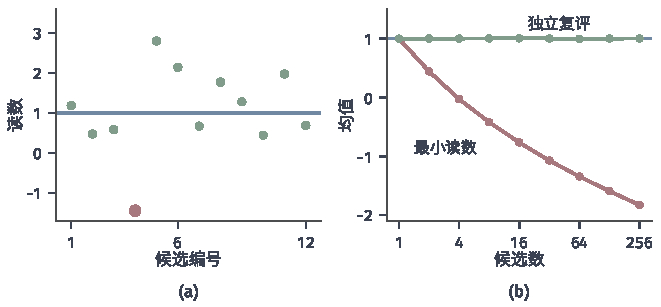
\includegraphics[width=112mm]{figures/05-optimization/05-stochastic-optimization/matplotlib/zo-selection/figure.pdf}
  \caption{含噪比较的选择偏差，真实值都是$1$（蓝线），噪声为标准正态。(a)$12$个候选的一次读数，红点是读数最低者，它并不比其他候选好。(b)红线是$K$个候选中最小读数的均值，随$K$增大而偏低；绿线是选定后独立复评的均值，始终等于真值。每点$10^5$次模拟。}
  \label{fig:zo-selection}
\end{BookInlineFigure}
